% !TeX spellcheck = ru_RU
\section{Дискретное преобразование Фурье}
Дискретное преобразование Фурье (ДПФ) --- инструмент спектрального анализа сигналов. ДПФ позволяет сопоставить сигналу во временной области эквивалентное представление в частотной области.
Данное преобразование ставит в соответствие \(N\) отсчетам сигнала \(s(n), n = 0, 1 \dots N-1,  N\) отсчетов комплексного \(S_d(k), k = 0 \dots N-1 \).

Для того, что бы понять принцип работы ДПФ рассмотрим модель приемника, изображенного на
рисунке~\ref{fig:vol_recieverDFT}.

Сигнал, поступающий на вход приемника, умножается на базовые функции \(sin\) и \(cos\) различных
частот. Таким образом определяются частоты, присутствующие в сигнале. Более того, данные частоты
ортогональны друг другу, т.е. их скалярное умножение равно 0.
\begin{figure}[H]
    \centering
    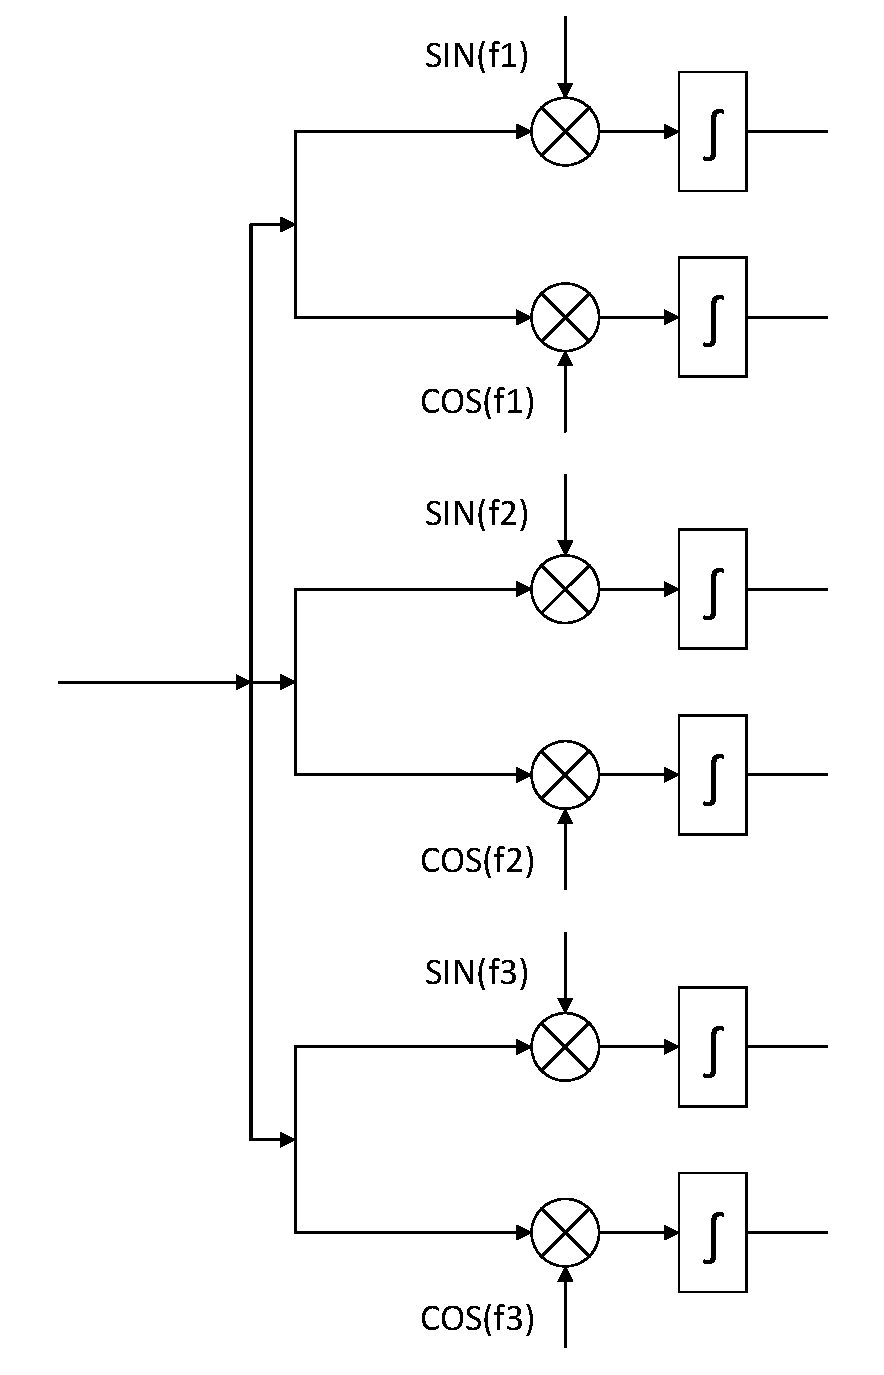
\includegraphics[width=0.5\textwidth]{img/vol_recieverDFT}
    \caption{ДПФ в приемнике}
    \label{fig:vol_recieverDFT}
\end{figure}

Формула прямого преобразования имеет следующий вид:
\begin{equation}
    S(k) = \sum_{n=0}^{N-1} s(n) \cdot e^{-j \cdot \dfrac{2\pi}{N} \cdot n \cdot k}, k = 0 \dots N-1
\end{equation}

Согласно формуле Эйлера \(e^{jx} = \cos(x) + j\sin(x)\) преобразование Фурье может быть представлено в следующем виде:
\begin{equation} \label{eq:DFT_cos}
    S(k) = \sum_{n=0}^{N-1} s(n) \cdot (\cos(\dfrac{2\pi}{N} \cdot n \cdot k) - j \sin(\dfrac{2\pi}{N} \cdot n \cdot k))
\end{equation}

Рассмотрим пример использования ДПФ над дискретным сигналом из 8-ми отсчетов (\(N = 8, n = [0:7]\)).

Сигнал задается следующим выражением: \[s(n) = cos(2 \cdot \pi \cdot n \cdot k / N) + j \cdot
sin(2 \cdot \pi \cdot n \cdot k / N) \].

Если задать k = 0, то сигнал будет постоянным. \[s(n) = cos(2 \cdot \pi \cdot n \cdot 0 / N) + j \cdot sin(2 \cdot \pi \cdot n \cdot 0 / N) = cos(0) - j \cdot sin(0) = 1\]
При выполнении процедуры дискретного преобразования Фурье над таким сигналом будет произведены
следующие вычисления:\newline
\(S(k = 0): \sum_{n=0}^{N = 8} (cos(0) + j \cdot sin(0)) \cdot (cos(0) - j \cdot sin(0) =
\sum_{n=0}^{N = 8} 1 \) \newline
\(S(k = 1): \sum_{n=0}^{N = 8} (cos(2 \cdot \pi \cdot n/N) - j \cdot sin(2 \cdot \pi\cdot n/N))
=\sum_{n=0}^{N = 8} 0 \) \newline
\(S(k = 2): \sum_{n=0}^{N = 8}  (cos(2 \cdot \pi \cdot 2 \cdot n/N) - j \cdot sin(2 \cdot \pi \cdot
2\cdot n/N)) = \sum_{n=0}^{N = 8} 0 \) \newline
\dots \newline
\(S(k = 7): \sum_{n=0}^{N = 8} (cos(2 \cdot \pi \cdot 7 \cdot n/N) - j \cdot sin(2 \cdot \pi \cdot
7\cdot n/N)) = \sum_{n=0}^{N = 8} 0 \) \newline

Как видно из приведенных вычислений, после применения ДПФ, будет получен сигнал с единственной частотой
в k = 0. Остальные частоты равны 0, потому что частота сигнала ортогональна всем базовым частотам
преобразования. На рисунке~\ref{fig:vol_DFT_k3} приведен пример умножения сигнала на базовые функции
синуса и косинуса при k = 3.
\begin{figure}[H]
    \centering
    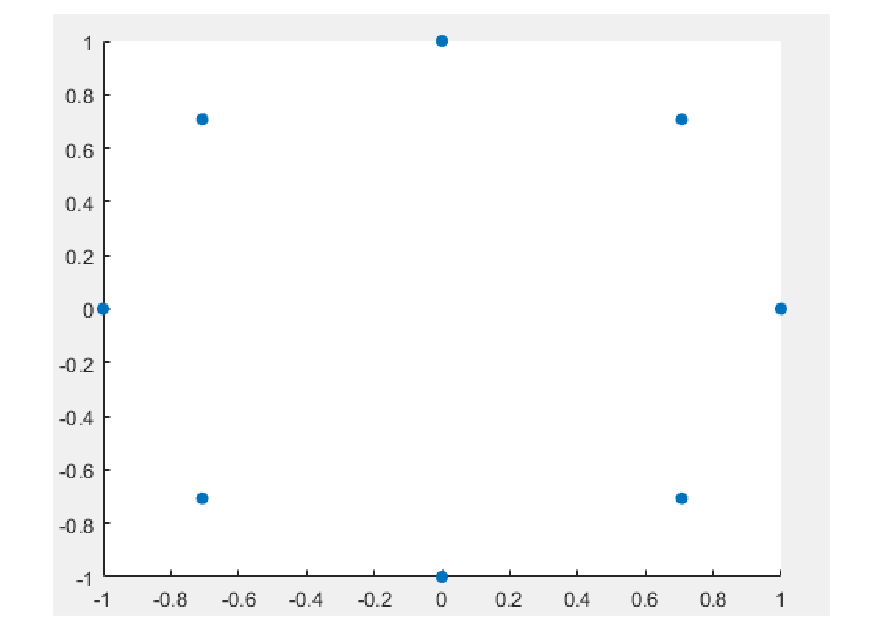
\includegraphics[width=0.5\textwidth]{img/vol_DFT_k3}
    \caption{Умножение сигнала на базовые функции. k=3.}
    \label{fig:vol_DFT_k3}
\end{figure}
Сложив данный ряд чисел, получится 0, так как каждая точка имеет противоположную.

Таким образом, задав входной ДПФ сигнал с помощью выражения \(cos(2 \cdot \pi \cdot n \cdot k / N) + j \cdot sin(2 \cdot \pi \cdot n \cdot k / N) \) и изменяя k, можно указывать необходимую частоту на
выходе блока ДПФ. Если входной сигнал задать как сумма подобных выражений с различными k, то на выходах
блока ДПФ, с указанными k, частоты будут не нулевыми.

Обратное преобразование Фурье позволяет сопоставить сигналу в частотной области эквивалентное представление во временной области.

Формула обратного преобразования имеет следующий вид:
\begin{equation}
s(n) = \dfrac{1}{N}\cdot \sum_{k=0}^{N-1} S(k) \cdot e^{j \cdot \dfrac{2\pi}{N} \cdot n \cdot k}, k = 0 \dots N-1
\end{equation}
Функция обратного преобразования идентична функции прямого преобразования. Отличие состоит лишь в
степени комплексной экспоненты, которая является комплексно сопряженной к экспоненте прямого
преобразования. Данный факт позволяет производить обратное преобразование на прямом. Для этого
достаточно подать на вход ОДПФ комплексно-сопряженный сигнал.

Покажем, что при применении результата ПДПФ к ОДПФ получится исходный сигнал:\newline
\(s(n) = \sum_{n = 0}^{N -1} s(n) \cdot (\cos(\dfrac{2\pi}{N} \cdot n \cdot k) - j \sin(\dfrac{2\pi}{N}
\cdot n \cdot k)) \cdot (\cos(\dfrac{2\pi}{N} \cdot n \cdot k) + j \sin(\dfrac{2\pi}{N} \cdot n \cdot
k)) = \sum_{n = 0}^{N -1} s(n) \cdot \cos^2(\dfrac{2\pi}{N} \cdot n \cdot k) - j^2 \cdot
\sin^2(\dfrac{2\pi}{N} \cdot n \cdot k)) = \sum_{n = 0}^{N -1} s(n) \cdot 1\).

Для получения на выходе ОДПФ сигналов, например синусоиды, нужно подать на вход ряд
комплексных чисел, мнимая часть которых будет отлична от нуля. Более того, те индексы k, которые будут
не нулевыми и зададут частоту итоговой синусоиды.